\documentclass[conference]{IEEEtran}
\IEEEoverridecommandlockouts
% The preceding line is only needed to identify funding in the first footnote. If that is unneeded, please comment it out.
\usepackage{cite}
\usepackage{amsmath,amssymb,amsfonts}
\usepackage{algorithmic}
\usepackage{graphicx}
\usepackage{textcomp}
\usepackage{xcolor}
\def\BibTeX{{\rm B\kern-.05em{\sc i\kern-.025em b}\kern-.08em
    T\kern-.1667em\lower.7ex\hbox{E}\kern-.125emX}}
\begin{document}

\title{Paper Title*\\
\thanks{Identify applicable funding agency here. If none, delete this.}
}

\author{\IEEEauthorblockN{1\textsuperscript{st} Given Name Surname}
\IEEEauthorblockA{\textit{dept. name of organization (of Aff.)} \\
\textit{name of organization (of Aff.)}\\
City, Country \\
email address}
\and
\IEEEauthorblockN{2\textsuperscript{nd} Given Name Surname}
\IEEEauthorblockA{\textit{dept. name of organization (of Aff.)} \\
\textit{name of organization (of Aff.)}\\
City, Country \\
email address}
\and
\IEEEauthorblockN{3\textsuperscript{rd} Given Name Surname}
\IEEEauthorblockA{\textit{dept. name of organization (of Aff.)} \\
\textit{name of organization (of Aff.)}\\
City, Country \\
email address}
\and
\IEEEauthorblockN{4\textsuperscript{th} Given Name Surname}
\IEEEauthorblockA{\textit{dept. name of organization (of Aff.)} \\
\textit{name of organization (of Aff.)}\\
City, Country \\
email address}
\and
\IEEEauthorblockN{5\textsuperscript{th} Given Name Surname}
\IEEEauthorblockA{\textit{dept. name of organization (of Aff.)} \\
\textit{name of organization (of Aff.)}\\
City, Country \\
email address}
\and
\IEEEauthorblockN{6\textsuperscript{th} Given Name Surname}
\IEEEauthorblockA{\textit{dept. name of organization (of Aff.)} \\
\textit{name of organization (of Aff.)}\\
City, Country \\
email address}
}

\maketitle

\begin{abstract}
With falls being at the same time more susceptible in advanced ages and the second most common cause of accidental death to elders, detecting falls became a necessary research topic to an aging population~\cite{who2007report}. To this effect, we proposed and evaluated the employment of a multi-stream approach to detect fall events. Three features (optical flow, saliency map, and RGB data) fed to each stream of a VGG-16 and classified by an SVM of whether there was or not a fall event. We experimented on two datasets URFD and FDD, achieving respectively 98.84\% and 99.51\% accuracy, outperforming the majority of reviewed solutions.
\end{abstract}

\begin{IEEEkeywords}
Multi-stream, optical flow, saliency, video, deep learning
\end{IEEEkeywords}

\section{Introduction}

With deteriorating health in advanced ages, even a minor fall can trigger a chain reaction of serious psychological and physical injuries to the elder population. Hence, the motivation for ambient assistant living solutions to both avoids falling from occurring and reducing the interval between a fall and help arrival. The studies conducted to detect falls as soon as they happen can be split into two main categories. Hardware reliant solutions, such as accelerometers and IMUs. Which are met with frustration from the subjects, mainly towards forgetting to use the device, despite their fall detection performance. And vision-based solutions, which allied to machine learning techniques have shown promising results and, furthermore, not relying on the subject's set up to operate.

Throughout the fall detection literature, techniques vary from threshold activation based, such as Sase et al.~\cite{sase2018human} detecting regions of interest after background subtraction, and a threshold activation function if the region of interest was under a third of the subject height in the frame. Bhandari et al.~\cite{bhandari2017novel} determined regions of interest via Shi-Tomasi, tracked them using Lucas-Kanade and set a threshold on the region of interest's speed and motion. And Albawendi et al.~\cite{albawendi2018video} who used a threshold activation on silhouette shape. Another commonly used classification technique is support vector machine (SVM), used by Harrou et al.~\cite{harrou2017vision} that fed a feature extractor with the subject segmented from the frame. They compared extractor output with a multivariate exponentially-weighted moving average (MEWMA) and classified by an SVM. Panahi et al.~\cite{panahi2018human} subtracted the background from depth images, fitted an ellipse in the subject's shape, and classified it with SVM. Abobakr et al.~\cite{abobakr2017skeleton} also subtracted the background from depth images, applied a random decision forest to estimate the subject's posture, and an SVM to classify it. Regarding the subject's privacy, both Edgcomb et al.~\cite{edgcomb2012automated} and Lin et al.~\cite{lin2013fall} investigated privacy-prone features, such as blurring, silhouetting, and covering the body with shapes. Lu et al.~\cite{lu2018deep} employed a 3D convolutional neural network (CNN) followed by a long short-term memory (LSTM). Huang et al.~\cite{huang2018video} extracted the human pose with OpenPose and classified it with a VGG-16 architecture. N\'u\~nez-Marcos et al.~\cite{nunez2017vision} extracted the dense optical flow (OF) and also served it to a VGG-16. And Anishchenko et al.~\cite{anishchenko2018machine} employed a modified AlexNet as a classifier. A few different approaches were also reported, such as K-nearest neighbor classifiers by Sehairi et al.~\cite{sehairi2018elderly} and Kwolek et al.~\cite{kwolek2015improving}. Hidden Markov model by Zerrouki et al.~\cite{zerrouki2018combined} and Qian et al.~\cite{qian2017recognizing}. Particle filtering by Yu et al.~\cite{yu2009fall}. And Gaussian models by Yu et al.~\cite{yu2010robust} and Rougier et al.~\cite{rougier2011robust}. Furthermore, Xu et al.~\cite{xu2018new} produced a survey on fall detections systems.

This work's main contribution is the development and evaluation of hand-crafted features in a multi-stream learning model. To this end, we compare the effectiveness of three features extracted from videos frames: (i) optical flow, (ii) saliency map, and (iii) RGB features. These features a fed to a three-stream VGG-16 architecture, and their results compared with the literature.

We organized this paper as follows. In Section~\ref{sec:method} we detail the proposed three-stream methodology. In Section~\ref{sec:experiments} we performed experiments and compared their results to other works in the literature. Moreover, in Section~\ref{sec:conclusion} we elaborate on some points and future work suggestions.

\section{Background}
\label{background}

In this section, we describe a few relevant concepts employed in Section~\ref{sec:method}.

\subsection{Optical Flow}
\label{sec:opticalflow}

Optical flow is a hand-crafted feature that conveys movement information between two frames of a video, either by object or camera movement. Its ability to describe movement enables this feature to support the temporal aspect of a fall event in a deep network.

The extraction process considers a video frame as $I$ and $I(x, y, t)$ a pixel in this frame. Another frame collected $dt$ time later, and the distance that the same pixel moved $(dx, dy)$ is described in Equation~\ref{eq:of-dist}.

Optical flow's Equation~\ref{eq:of} is formed after applying a Taylor series approximation of right-hand side and dividing by $dt$, $f_t$ is the gradient given time, $f_x$, $f_y$, $u$, and $v$ are given in Equation~\ref{eq:of-grad}. Values of $u$ and $v$ can be achieved by different methods, such as the classical Lucas-Kanade~\cite{jain2018abnormal} or the one used in this work: Gunnar-Farneb{\"a}ck~\cite{lowhur2015dense}.

\begin{equation}
\label{eq:of-dist}
I(x, y, t)=I(x+dx, y+dy, t+dt)
\end{equation}
\begin{equation}
\label{eq:of}
f_xu + f_yv + f_t=0
\end{equation}
\begin{equation}
\label{eq:of-grad}
f_x = \frac{\partial f}{\partial x}; \quad f_y = \frac{\partial f}{\partial y}u = \frac{\partial x}{\partial t}; \quad v = \frac{\partial y}{\partial t}
\end{equation}

\subsection{Saliency Map}
\label{sec:saliency}

Envisioned as a visualizing technique to understand the learning process behind a deep network. Its extraction can occur in many ways, one of those being the practice of feeding an image $I$ and its class label $c$ to the network, then, freezing the weights on the network and compute the gradients of $c$ to the pixels of $I$. Consider $S_c(I)$ to be the class score function for an image $I$ and, for this simple explanation, that it is a simple linear function, $S_c(I) = w_c^{T} + b_c$. With $w$ being the weights of the network and $b$ the bias, it is possible to notice that the magnitude of elements of $w$ affects the importance of the corresponding pixels in $I$ with class $c$.

The choice of saliency map as a stream is due to its spatial relation to the frame, as the raw RGB frames are prone to environmental interference, and its performance in the works of Zuo et al.~\cite{zuo2019enhanced} and Meng et al.~\cite{Meng2018interpretable}. We applied Sundararajan's et al.~\cite{sundararajan2017axiomatic} saliency method in this work.

\section{Method}
\label{sec:method}

As further detailed below, to classify between fall and not fall in video sequences we used an ensemble of VGG-16s and evaluated them,  Figure~\ref{fig:overview} shows an overview of the method.

\begin{figure}[htbp]
\centerline{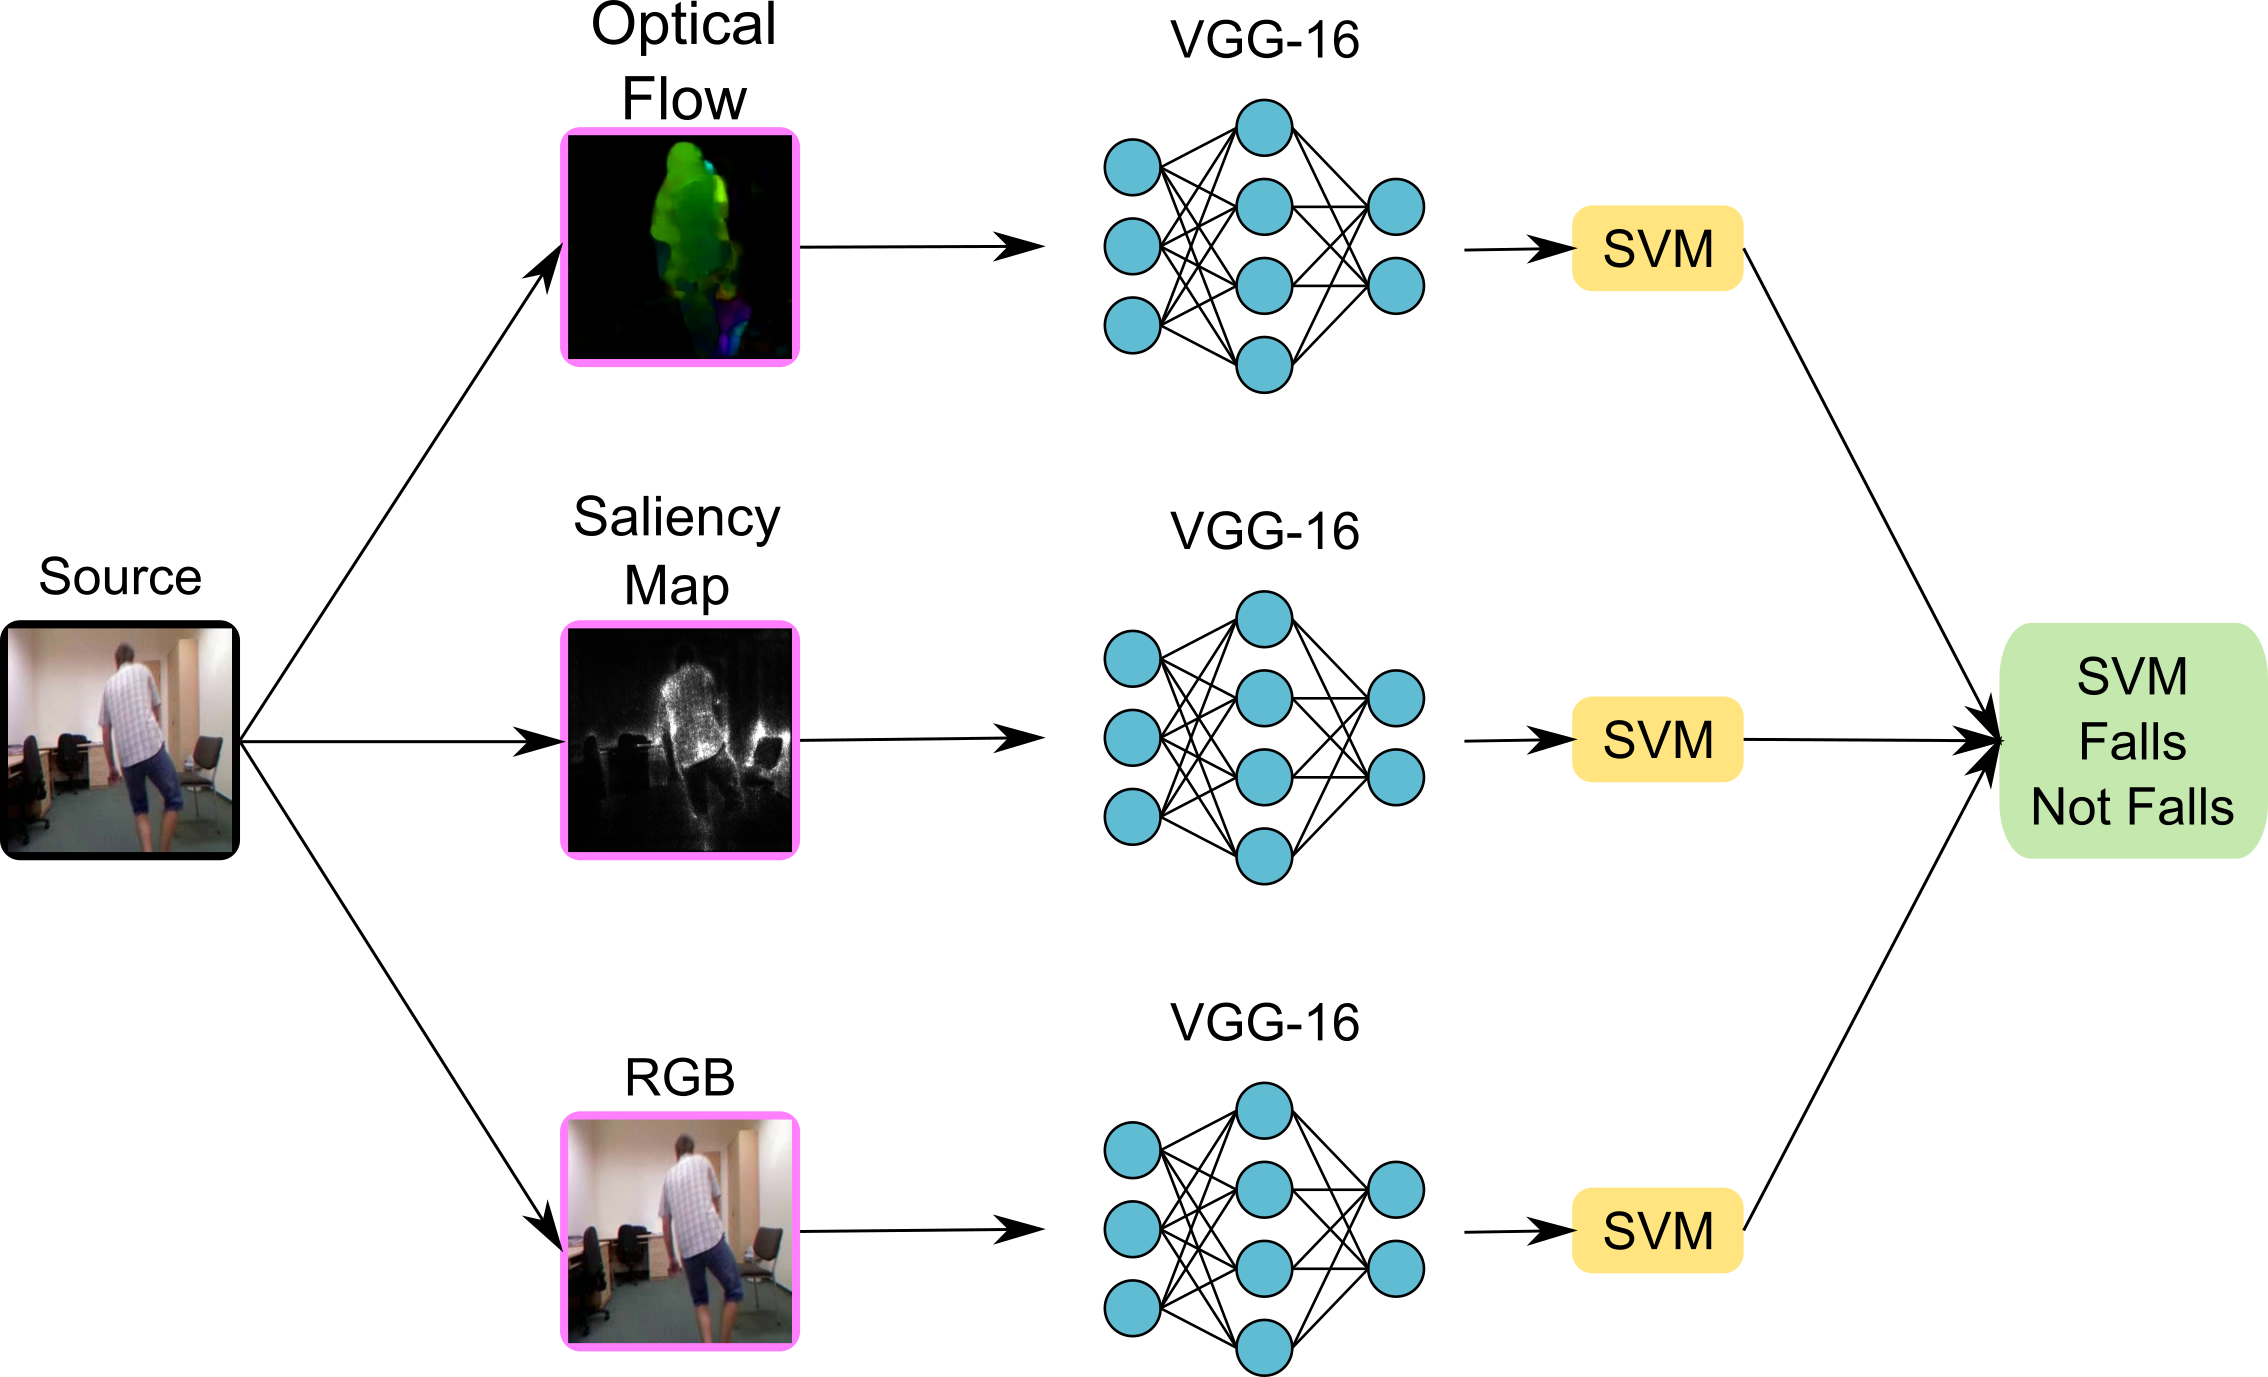
\includegraphics[width=\linewidth]{figures/overview.png}}
\caption{Methodology overview.}
\label{fig:overview}
\end{figure}

\subsection{Transfer Learning}

The selected datasets, further detailed in Section~\ref{sec:experiments}, possess relatively few human fall samples in their videos, which would limit the CNNs learning capabilities to detect fall events. Hence, the importance of transfer learning.

The first 14 layers of the VGG-16 architecture were trained on the ImageNet~\cite{imagenet_cvpr09} dataset, and later on, these same layers were fine-tuned over the UCF101~\cite{soomro2012ucf101} dataset. The reasoning being that the network would initially learn low-level features from the ImageNet classes, and focus these features on human activities with the UCF101 videos, Figure~\ref{fig:pre14}. N\'u\~nez-Marcos et al.~\cite{nunez2017vision} executed this step and released their weights files publicly.

\begin{figure}[htbp]
\centerline{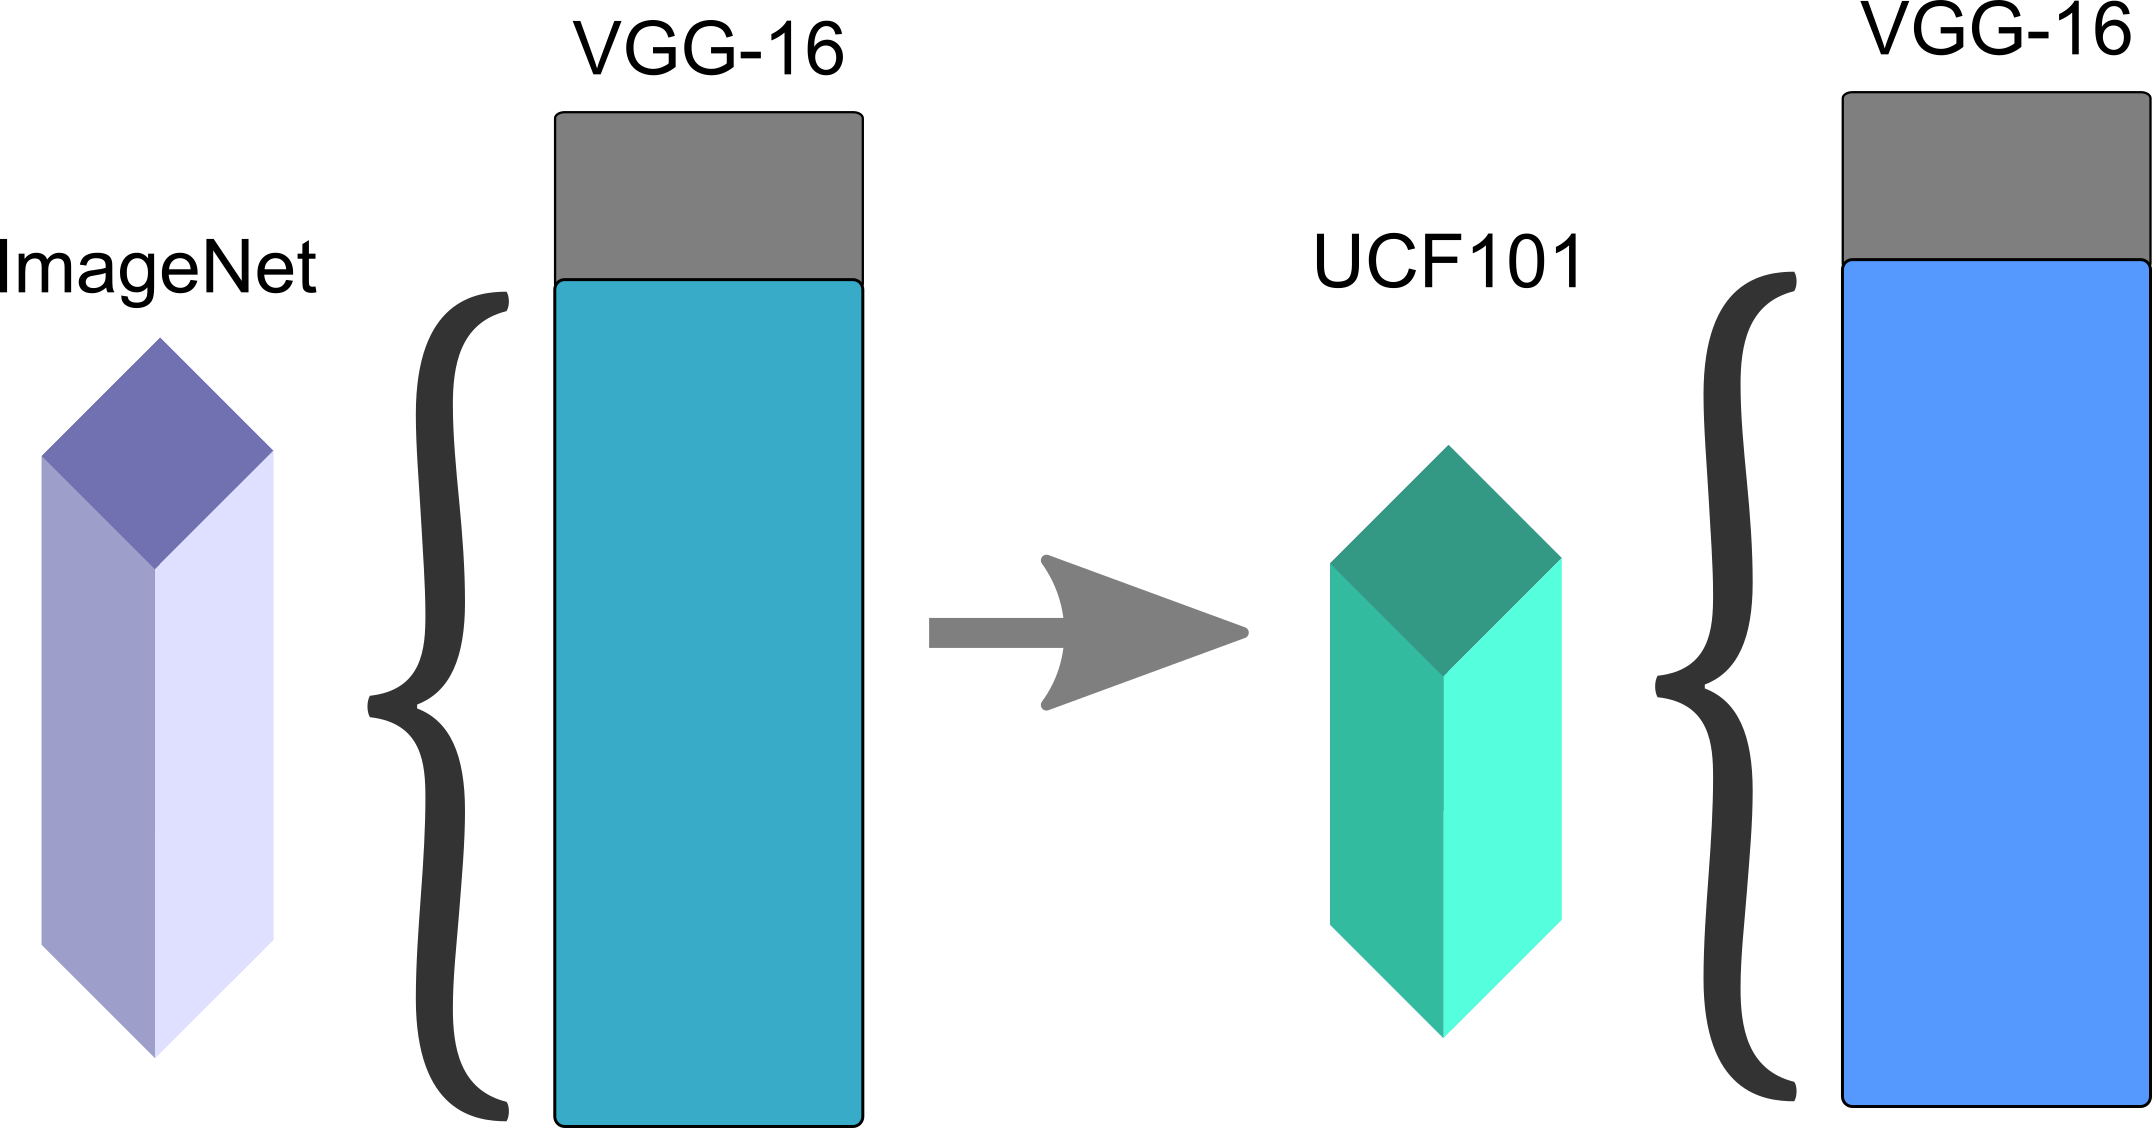
\includegraphics[width=0.9\linewidth]{figures/pre14.png}}
\caption{Deep layers being trained by ImagetNet and UCF101.}
\label{fig:pre14}
\end{figure}

We froze the 14 initial layer's weights and fine-tuned the last two fully connected layers were fine-tuned, with dropout regularization. Each stream executed this last fine-tuning step, totaling three executions, Figure~\ref{fig:pos14}.

\begin{figure}[htbp]
\centerline{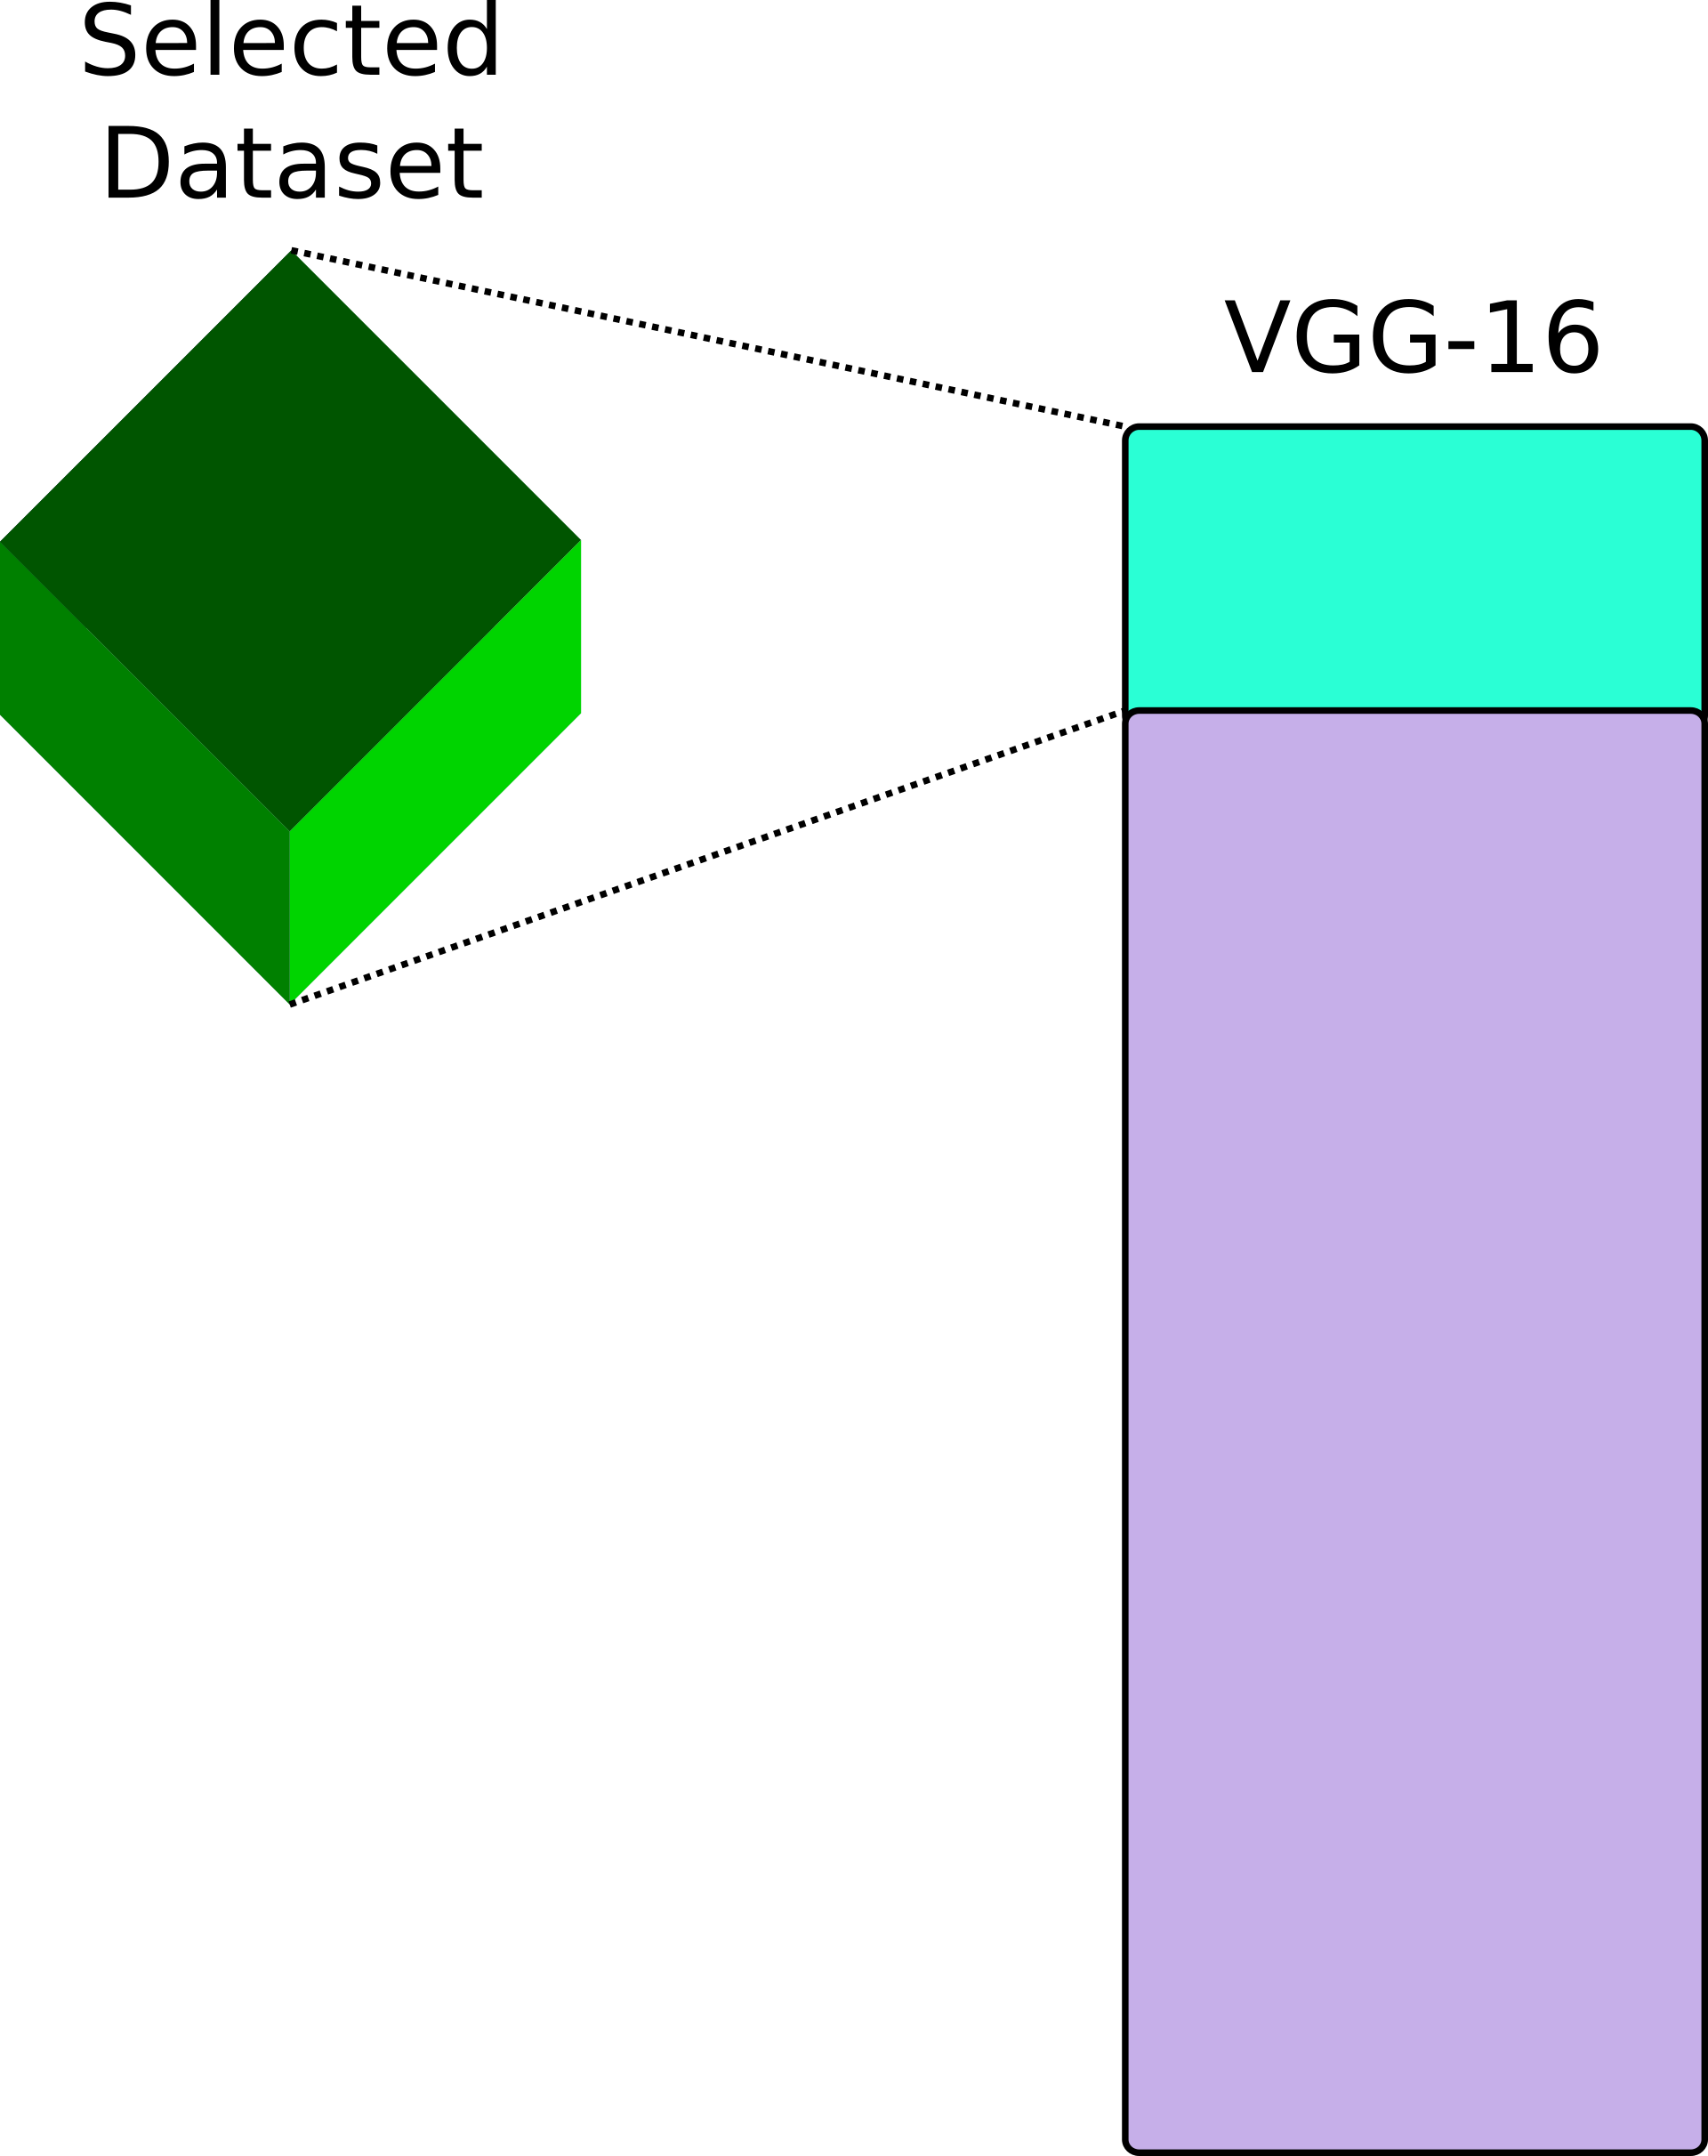
\includegraphics[width=0.4\linewidth]{figures/pos14.png}}
\caption{Fully connected layers training.}
\label{fig:pos14}
\end{figure}

\subsection{Classification}
\label{sec:classification}

Wang et al.~\cite{wang2015towards} reported that networks employing multi-stream classifiers outperformed their single-streamed peers. Inspired on this finding, an SVM classifier fed with the outputs of each stream, vectors between 0 and 1, generates a ($x$, $y$, $z$) vector. A second SVM uses this vector to classify between fall and not fall, Figure~\ref{fig:overview}.

\subsection{Streams Input}

The features Optical Flow and Saliency map were fed to the streams we explained in Subsection~\ref{sec:classification}, and furthermore, given the neural networks capability to learn relevant features to describe their input, the RGB frame itself was fed to the third stream.

\paragraph{Optical Flow} represents the temporal relation between frames, and to fully gather this property it was used as a stack of optical flows on top of a sliding window of frames, as suggested by N\'u\~nez-Marcos et al.~\cite{nunez2017vision}. The sliding window has a size of $L$ frames and gathers 2$L$ components ($L$ horizontal ($d_t^x$) + $L$ vertical ($d_t^y$) optical flow component vector fields) creating a stack $O$ = \{$d_t^x$, $d_t^y$, $d_{t+1}^x$, $d_{t+1}^y$, ..., $d_{t+L}^x$, $d_{t+L}^y$ \}. The total number of stacks is given by $N$-$L$+$1$, where $N$ is the number of frames in a video, Figure~\ref{fig:of} shows and extracted example.
\paragraph{Saliency Map} is composed of pixels varying from 0 to 1, and was fed as a gray-scale image to the network, Figure~\ref{fig:sal} shows and extracted example.

\begin{figure}[htbp]
\centerline{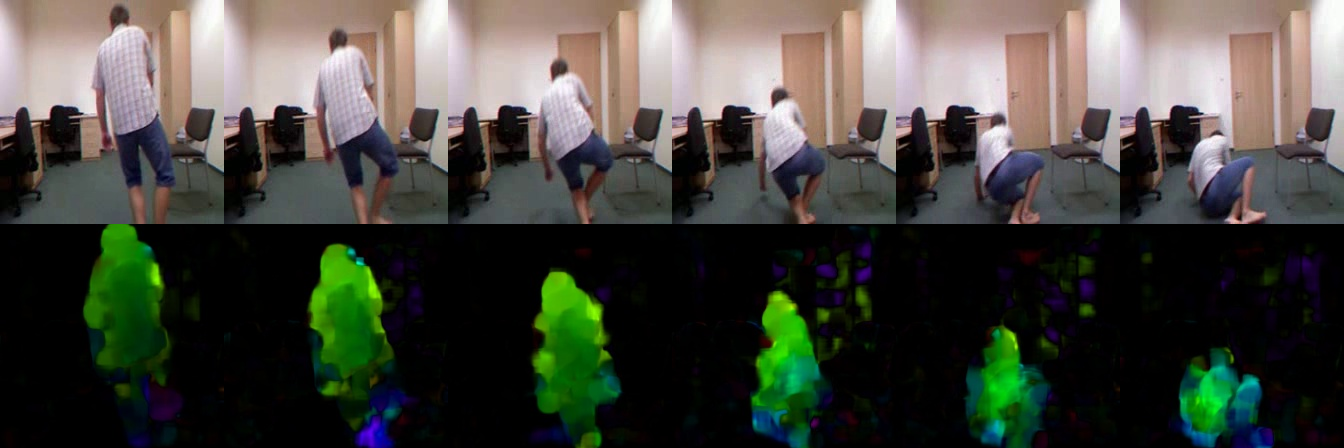
\includegraphics[width=\linewidth]{figures/of.png}}
\caption{A frame and its extracted optical flow.}
\label{fig:of}
\end{figure}

\begin{figure}[htbp]
\centerline{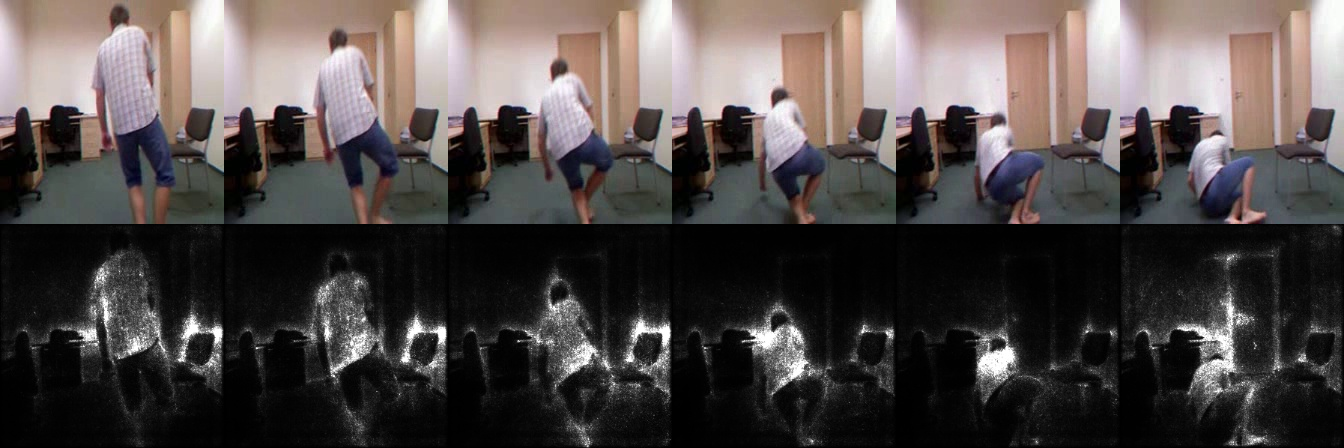
\includegraphics[width=\linewidth]{figures/sal.png}}
\caption{A frame and its extracted saliency map.}
\label{fig:sal}
\end{figure}

\section{Experiments}
\label{sec:experiments}

Our experiments were performed on two publicly available datasets, \textit{URFD}~\cite{kepski2014human} and \textit{FDD}~\cite{charfi2013optimised}.

\paragraph{URFD dataset} contains 70 videos: (i) 30 videos of falls; and (ii) 40 videos of daily living activities, recorded from a top-down and front view perspective by two Microsoft Kinect cameras. Each frame is labeled in three categories, if the person is lying on the ground, not lying on the ground, and in an intermediate pose.
\paragraph{FDD dataset} is composed of 191 videos of which 143 are falls, recorded from a surveillance camera perspective by a single RGB camera. With every frame annotated between fall and not fall.

For the sake of comparison with other works we evaluated our method by three metrics: (i) Sensitivity reflecting the true positive rate, (ii) Specificity also known as the true negative rate, and (iii) Accuracy representing the overall performance of the method. We used a learning rate of $10^{-4}$, 500 epochs, 5-fold cross-validation, mini-batches of $2^{10}$, and Adam optimization. We also experimented with different classes weights, however, further tuning of the hyper-parameters we were able to keep both classes on the same weight. As explained in Section~\ref{sec:classification}, a double SVM is used to ensemble the outputs.

Tables~\ref{tab:urfd-ensem} and~\ref{tab:urfd-our-their} shows the results obtained over the URFD dataset. In Table~\ref{tab:urfd-ensem} we compare each single-stream feature with their multi-stream counterpart. The optical flow single-stream acquired the highest accuracy, at 97.57\%, and the multi-stream was still able to outperform it, at 98.84\%. Table~\ref{tab:urfd-our-their} compares our result with other works in the literature, whilst not all works measured their sensitivity and specificity, all of them reported their accuracy. Our method's accuracy and specificity performed better than most and kept the same 100\% sensitivity. Lu et al.~\cite{lu2018deep} was the only work to perform better than ours, and we believe the reason for such is the temporal importance to detect a fall event, and their usage of LSTM would better cater this relationship.

\begin{table}[]
\centering
\caption{URFD single-stream \textit{vs} multi-stream, decreasing accuracy.}
\label{tab:urfd-ensem}
\begin{tabular}{llcccl}
\hline
 &  & Sens. (\%) & Spec. (\%) & Acc. (\%) &  \\ \hline
 & OF + RGB + Sal & \textbf{100} & \textbf{98.77} & \textbf{98.84} &  \\
 & Optical Flow & \textbf{100} & 97.42 & 97.57 &  \\
 & RGB & \textbf{100} & 96.35 & 96.56 &  \\
 & Saliency & 93.67 & 93.39 & 93.40 &  \\ \hline
\end{tabular}
\end{table}

\begin{table*}[]
\centering
\caption{URFD our method \textit{vs} literature, decreasing accuracy.}
\label{tab:urfd-our-their}
\begin{tabular}{llcccl}
\hline
 &                                                      & Sensitivity (\%)  & Specificity (\%)  & Accuracy (\%)     & \\ \hline
 & Lu et al.~\cite{lu2018deep}                          & -                 & -                 & \textbf{99.27}    & \\
 & Ours                                                 & \textbf{100}      & \textbf{98.77}    & 98.84             & \\
 & Panahi et al.~\cite{panahi2018human}                 & 97.05             & 97.02             & 97.14             & \\
 & Zerrouki and Houacine~\cite{zerrouki2018combined}    & -                 & -                 & 96.88             & \\
 & Harrou et al.~\cite{harrou2017vision}                & -                 & -                 & 96.66             & \\
 & Abobakr et al.~\cite{abobakr2017skeleton}            & \textbf{100}      & 0.91              & 96.00             & \\
 & Bhandari et al.~\cite{bhandari2017novel}             & 96.66             & -                 & 95.71             & \\
 & Kwolek and Kepski~\cite{kwolek2015improving}         & \textbf{100}      & 92.50             & 95.71             & \\
 & N\'u\~nez-Marcos et al.~\cite{nunez2017vision}       & \textbf{100}      & 92.00             & 95.00             & \\
 & Sase et al.~\cite{sase2018human}                     & 81.00             & -                 & 90.00             & \\ \hline
\end{tabular}
\end{table*}

Tables~\ref{tab:fdd-ensem} and~\ref{tab:fdd-our-their} reports the results extracted from the FDD dataset. Homologous to the URFD report, Table~\ref{tab:fdd-ensem} compares each single-stream with the multi-stream approach. The multi-stream achieved 99.51\% accuracy, and the highest single-stream score was again the optical flow, with 99.11\%. When comparing our results with the literature, in Table~\ref{tab:fdd-our-their}, our's outperformed every other one, regarding accuracy and sensitivity. And was 0.05\% worse then Charfi's et al.~\cite{charfi2013optimised} specificity. Our results also confirmed the findings of Wang et al.~\cite{wang2015towards} since each feature stream did not perform great on their own, but when applied together they contributed to state of the art results towards fall detection.

\begin{table}[]
\centering
\caption{FDD single-stream \textit{vs} multi-stream, decreasing accuracy.}
\label{tab:fdd-ensem}
\begin{tabular}{llcccl}
\hline
 &  & Sens. (\%) & Spec. (\%) & Acc. (\%) &  \\ \hline
 & OF + RGB + Sal & \textbf{99.43} & \textbf{99.55} & \textbf{99.51} &  \\
 & Optical Flow & 99.07             & 99.12             & 99.11             &  \\
 & RGB & 98.85             & 98.41             & 98.55             &  \\
 & Saliency & 88.39             & 92.40             & 91.25             & \\ \hline
\end{tabular}
\end{table}

\begin{table*}[]
\centering
\caption{FDD our method \textit{vs} literature, decreasing accuracy.}
\label{tab:fdd-our-their}
\begin{tabular}{llcccl}
\hline
 &                                                      & Sensitivity (\%)  & Specificity (\%)  & Accuracy (\%)     & \\ \hline
 & Ours                                                 & \textbf{99.43}    & 99.55             & \textbf{99.51}    & \\
 & Lu et al.~\cite{lu2018deep}                          & -                 & -                 & 99.36             & \\
 & Sehairi et al.~\cite{sehairi2018elderly}             & -                 & -                 & 98.91             & \\
 & Zerrouki and Houacine~\cite{zerrouki2018combined}    & -                 & -                 & 97.02             & \\
 & Harrou et al.~\cite{harrou2017vision}                & -                 & -                 & 97.02             & \\
 & Charfi et al.~\cite{charfi2012definition}            & 98.0              & \textbf{99.60}    & -                 & \\
 & N\'u\~nez-Marcos et al.~\cite{nunez2017vision}       & 99.0              & 97.00             & 97.00             & \\ \hline
\end{tabular}
\end{table*}
 
\section{Conclusion and Future Work}
\label{sec:conclusion}

This paper proposes to detect human fall events, based on the employment of a multi-stream convolutional neural network. Each stream was served an extracted feature, them being: (i) optical flow, (ii) saliency map, and (iii) the RGB frame itself, the double SVM performed the ensemble approach. e tested the proposed method on URFD and FDD datasets, and our solution outperformed the related literature in most cases, indicating that multi-stream approaches and the selected features can be useful to detect human fall events.

It is worth discussing the selected features and some literature results. As et al.~\cite{chernbumroong2012elderly} noted that privacy concerns might arise on video-based approaches, the selected features can conceal one's identity. Despite these feature's performance, both optical flow and saliency map are timely and computationally intensive to extract, which would halt their implementation in a real-time system. Considering this work's goal in exploring features to the fall detection problem, it is relevant to weight their extraction process against their results. And regarding other works in the literature, some seemed to dismiss the importance of the sensitivity metric, which quantifies the avoidance of false negatives. A World Health Organization report~\cite{who2007report}, enlightens the severity of an elderly fall, thus the importance of a high sensitivity metric.

Observing the results in Table~\ref{tab:urfd-our-their} and~\ref{tab:fdd-our-their}, it is possible to notice a saturation of these datasets, and as also reported by et al.~\cite{chernbumroong2012elderly}, systems trained on artificial environments did not perform as well on real-life scenarios. Therefore, the importance of future work to come up with a more extensive dataset that better resembles the actual application setup, Mastorakis et al.~\cite{mastorakis2018fall} published a simulated dataset of fall events. Method wise, as explained above, the exploration of cheaper features and deep networks that could generate comparable results, should also be focused on.

\section*{Acknowledgment}

%\begin{thebibliography}{00}
%\end{thebibliography}

\bibliographystyle{IEEEtran}
\bibliography{paper}

\end{document}
